\documentclass[12pt]{article}
    \usepackage{longtable} %dla tablic większych od 1 strony
\usepackage{multirow}
\usepackage[hyphenbreaks]{breakurl}
\usepackage[hyphens]{url}
%różne pakiety matematyczne, warto przejrzeć dokumentację, muszą być powyżej ustawień językowych.
\usepackage{mathrsfs}   %Różne symbole matematyczne opisane w katalogu ~\doc\latex\comprehensive. Zamienia \mathcal{L} ze zwykłego L na L-transformatę.
\usepackage{eucal}      %Różne symbole matematyczne.
\usepackage{amssymb}    %Różne symbole matematyczne.
\usepackage{amsmath}    %Dodatkowe funkcje matematyczne, np. polecenie \dfac{}{} skladajace ulamek w trybie wystawionym (porównaj $\dfrac{1}{2}$, a $\frac{1}{2}$).

%język polski i klawiatura
\usepackage[polish]{babel}
\usepackage[OT4]{polski}
\usepackage[utf8]{inputenc}                       %Strona kodowa polskich znaków.
%obsługa pdf'a
\usepackage[pdftex,usenames,dvipsnames]{color}      %Obsługa kolorów. Opcje usenames i dvipsnames wprowadzają dodatkowe nazwy kolorow.
\usepackage[pdftex,pagebackref=false,draft=false,pdfpagelabels=false,colorlinks=true,urlcolor=blue,linkcolor=red,citecolor=green,pdfstartview=FitH,pdfstartpage=1,pdfpagemode=UseOutlines,bookmarks=true,bookmarksopen=true,bookmarksopenlevel=2,bookmarksnumbered=true,pdfauthor={Piotr Bladek},pdftitle={Praca dyplomowa},pdfsubject={Praca dyplomowa},pdfkeywords={transient recovery voltage trv},unicode=true]{hyperref}   %Opcja pagebackref=true dotyczy bibliografii: pokazuje w spisie literatury numery stron, na których odwołano się do danej pozycji.

%bibliografia
\usepackage[numbers,sort&compress]{natbib}  %Porządkuje zawartość odnośników do literatury, np. [2-4,6]. Musi być pod pdf'em, a styl bibliogfafii musi mieć nazwę z dodatkiem 'nat', np. \bibliographystyle{unsrtnat} (w kolejności cytowania).
\usepackage{hypernat}                       %Potrzebna pakietowi natbib do wspolpracy z pakietem hyperref (wazna kolejnosc: 1. hyperref, 2. natbib, 3. hypernat).

%grafika i geometria strony
\usepackage{extsizes}           %Dostepne inne rozmiary czcionek, np. 14 w poleceniu: \documentclass[14pt]{article}.
\usepackage[final]{graphicx}
\usepackage[a4paper,left=3.5cm,right=2.5cm,top=2.5cm,bottom=2.5cm]{geometry}

%strona tytułowa
\usepackage{zalaczniki/ustawienia/strona_tytulowa}

%inne
\usepackage[hide]{todo}                     %Wprowadza polecenie \todo{treść}. Opcje pakietu: hide/show. Polecenie \todos ma byc na koncu dokumentu, wszystkie \todo{} po \todos sa ignorowane.
\usepackage[basic,physics]{circ}            %Wprowadza środowisko circuit do rysowania obwodów elektrycznych. Musi byc poniżej pakietow językowych.
\usepackage[sf,bf,outermarks]{titlesec}     %Troszczy się o wygląd tytułów rozdziałów (section, subsection, ...). sf oznacza czcionkę sans serif (typu arial), bf -- bold. U mnie: oddzielna linia dla naglowku paragraph. Patrz tez: tocloft -- lepiej robi format spisu tresci.
\usepackage{tocloft}                        %Troszczy się o format spisu trsci.
\usepackage{expdlist}    %Zmienia definicję środowiska description, daje większe możliwości wpływu na wygląd listy.
\usepackage{flafter}     %Wprowadza parametr [tb] do polecenia \suppressfloats[t] (polecenie to powoduje nie umieszczanie rysunkow, tabel itp. na stronach, na ktorych jest to polecenie (np. moze byc to stroma z tytulem rozdzialu, ktory chcemy zeby byl u samej gory, a nie np. pod rysunkiem)).
\usepackage{array}       %Ładniej drukuje tabelki (np. daje wiecej miejsca w komorkach -- nie są tak ścieśnione, jak bez tego pakietu).
\usepackage{listings}    %Listingi programow.
\usepackage[format=hang,labelsep=period,labelfont={bf,small},textfont=small]{caption}   %Formatuje podpisy pod rysunkami i tabelami. Parametr 'hang' powoduje wcięcie kolejnych linii podpisu na szerokosc nazwy podpisu, np. 'Rysunek 1.'.
\usepackage{appendix}    %Troszczy się o załączniki.
\usepackage{floatflt}    %Troszczy się o oblewanie rysunkow tekstem.
\usepackage{here}        %Wprowadza dodtkowy parametr umiejscowienia rysunków, tabel, itp.: H (duże). Umiejscawia obiekty ruchome dokladnie tam gdzie są w kodzie źródłowym dokumentu.
\usepackage{makeidx}     %Troszczy się o indeks (skorowidz).

\usepackage{pdfpages} %do załączania dokumentów PDF
%nieużywane, ale potencjalnie przydatne
%\usepackage{sectsty}           %Formatuje nagłówki, np. żeby były kolorowe -- polecenie: \allsectionsfont{\color{Blue}}.
%\usepackage{version}           %Wersje dokumentu.
%\usepackage{fancyhdr}          %Dodaje naglowki jakie się chce.
%\usepackage{antyktor}          %Składa dokument przy użyciu Antykwy Toruńskiej.
%\usepackage{antpolt}           %Składa dokument przy użyciu Antykwy Półtawskiego.
%\usepackage[left]{showlabels}  %Pokazuje etykiety, ale kiepsko bo nie mieszcza sie na marginesie (można od biedy powiększyć margines w pakiecie geometry powyżej). Nie może być na górze (pakiet).

    % ------------------------------------------------------------------------
%   Kropki po numerach sekcji, podsekcji, itd.
%   Np. 1.2. Tytuł podrozdziału
% ------------------------------------------------------------------------
\makeatletter
    \def\numberline#1{\hb@xt@\@tempdima{#1.\hfil}}                      %kropki w spisie treści
    \renewcommand*\@seccntformat[1]{\csname the#1\endcsname.\enspace}   %kropki w treści dokumentu
\makeatother

% ------------------------------------------------------------------------
%   Numeracja równań, rysunków i tabel
%   Np.: (1.2), gdzie:
%   1 - numer sekcji, 2 - numer równania, rysunku, tabeli
%   Uwaga ogólna: o otoczeniu figure ma być najpierw \caption{}, potem \label{}, inaczej odnośnik nie działa!
% ------------------------------------------------------------------------
\makeatletter
    \@addtoreset{equation}{section} %resetuje licznik po rozpoczęciu nowej sekcji
    \renewcommand{\theequation}{{\thesection}.\@arabic\c@equation} %dodaje kropkę

    \@addtoreset{figure}{section}
    \renewcommand{\thefigure}{{\thesection}.\@arabic\c@figure}

    \@addtoreset{table}{section}
    \renewcommand{\thetable}{{\thesection}.\@arabic\c@table}
\makeatother

% ------------------------------------------------------------------------
% Tablica
% ------------------------------------------------------------------------
\newenvironment{tablica}[3]
{
    \begin{table}[!tb]
    \centering
    \caption[#1]{#2}
    \vskip 9pt
    #3
}{
    \end{table}
}

% ------------------------------------------------------------------------
% Dostosowanie wyglądu pozycji listy \todos, np. zamiast 'p.' jest 'str.'
% ------------------------------------------------------------------------
\renewcommand{\todoitem}[2]{%
    \item \label{todo:\thetodo}%
    \ifx#1\todomark%
        \else\textbf{#1 }%
    \fi%
    (str.~\pageref{todopage:\thetodo})\ #2}
\renewcommand{\todoname}{Do zrobienia...}
\renewcommand{\todomark}{~uzupełnić}

% ------------------------------------------------------------------------
% Definicje
% ------------------------------------------------------------------------
\def\nonumsection#1{%
    \section*{#1}%
    \addcontentsline{toc}{section}{#1}%
    }
\def\nonumsubsection#1{%
    \subsection*{#1}%
    \addcontentsline{toc}{subsection}{#1}%
    }
\reversemarginpar %umieszcza notki po lewej stronie, czyli tam gdzie jest więcej miejsca
\def\notka#1{%
    \marginpar{\footnotesize{#1}}%
    }
\def\mathcal#1{%
    \mathscr{#1}%
    }
\newcommand{\atp}{ATP/EMTP} % Inaczej: \def\atp{ATP/EMTP}

% ------------------------------------------------------------------------
% Inne
% ------------------------------------------------------------------------
\frenchspacing                      %nie pamiętam co to jest, ale używam
%\flushbottom                       %nie pamiętam co to jest, ale nie używam
%\raggedbottom                      %nie pamiętam co to jest, ale nie używam
\hyphenation{ATP/-EMTP}             %dzielenie wyrazu w żądanym miejscu
\setlength{\parskip}{3pt}           %odstęp pomiędzy akapitami
\linespread{1.2}                    %odstęp pomiędzy liniami (interlinia)
\setcounter{tocdepth}{4}            %uwzględnianie w spisie treści czterech poziomów sekcji
\setcounter{secnumdepth}{4}         %numerowanie do czwartego poziomu sekcji włącznie
\titleformat{\paragraph}[hang]      %wygląd nagłówków
{\normalfont\sffamily\bfseries}{\theparagraph}{1em}{}
%\definecolor{niebieski}{rgb}{0.0,0.0,0.5}

    \title{Wykorzystanie internetu rzeczy oraz bezzałogowych statków powietrznych przy wspomaganiu prowadzenia akcji ratunkowej}
    \author{Piotr Błądek}
    %polecenia zdefiniowane w pakiecie strona_tytulowa.sty
    \uczelnia{POLITECHNIKA WARSZAWSKA}
    \instytut{Instytut Elektrotechniki Teoretycznej i Systemów Informacyjno-Pomiarowych}
    \promotor{dr hab. inż. Piotr Biczel}
    \praca{Kierujący pracą: }
    \rok{2017}
    \usepackage{indentfirst}
\begin{document}
    \renewcommand{\figurename}{Rys.}    %musi byc pod \begin{document}, bo w~tym miejscu pakiet 'babel' narzuca swoje ustawienia
    \renewcommand{\tablename}{Tab.}     %j.w.
    \pagenumbering{roman}               %numeracja stron: rzymska
    \thispagestyle{empty}               %na tej stronie: brak numeru
    \stronatytulowa                     %strona tytułowa tworzona przez pakiet strona_tytulowa.tex

    \null\newpage

    %\input{zalaczniki/tekstowe/oswiadczenieDyplomant.tex}
    \newpage
\hfill \hfill Warszawa, dnia ................... roku \\
Politechnika Warszawska\\
Wydział Elektryczny
\vskip 1cm
\begin{center}
 {\large\bf  OŚWIADCZENIE} \\
\end{center}
\vskip 1cm
Świadomy odpowiedzialności prawnej oświadczam, że niniejsza praca dyplomowa magisterska pt. 
\textit{Wykorzystanie internetu rzeczy oraz bezzałogowych statków powietrznych przy wspomaganiu prowadzenia akcji ratunkowej:}
\begin{itemize}
\item została napisana przeze mnie samodzielnie
\item nie narusza niczyich praw autorskich 
\item nie zawiera treści uzyskanych w sposób niezgodny z obowiązującymi przepisami.
\end{itemize}
Oświadczam, że przedłożona do obrony praca dyplomowa nie była wcześniej podstawą postępowania związanego z uzyskaniem dyplomu lub tytułu zawodowego w uczelni wyższej. \\
Jestem świadom, że praca zawiera również rezultaty stanowiące własności intelektualne Politechniki Warszawskiej, które nie mogą być udostępniane innym osobom i instytucjom bez zgody Władz Wydziału Elektrycznego. \\
Oświadczam ponadto, że niniejsza wersja pracy jest identyczna z załączoną wersją elektroniczną. \\

\vskip 1cm
\noindent
\hfill \hfill (data i podpis dyplomanta)

    \newpage
    \newpage
\begin{center}
 {\large\bf  Streszczenie} \\
\vskip 1cm
Temat pracy:\\
\textit{\bf Wykorzystanie internetu rzeczy oraz bezzałogowych
statków powietrznych przy wspomaganiu prowadzenia
akcji ratunkowej}\\
\end{center}

Niniejsza praca, przedstawia proces tworzenia systemu wykorzystującego internet rzeczy i bezzałogowe statki powietrzne, przy wspomaganiu akcji ratowniczej. Zaczynam od wstępu teoretycznego, opisu technologii i sposobu w jaki chcę połączyć obie technologie, później przechodzę do swojej implementacji, opisu zastosowanych przeze mnie rozwiązań, problemów i ich rozwiązań, na koniec przedstawiam wyniki testów systemu i wnioski, jakie wyciągnąłem z tego projektu.

Temat jest trudny, trzeba połączyć dwie, dość nowe technologie, bezzałogowe statki powietrzne oraz internet rzeczy, tak żeby ze sobą współpracowały tworząc system, który z założenia ma pomagać ratownikom. Po drodze napotkałem wiele problemów, począwszy od bezpieczeństwa, przez autonomiczne sterowanie, krótki czas lotu UAV itd. Starałem się opisać, jak sobie z nimi radziłem.

W procesie tworzenia systemu powstało kilka programów, program na system Android, został zmodyfikowany program kontrolera lotu Pixhawk, oraz program stacji naziemnej w frameworku Django. Nie załączam tutaj kodu źródłowego, jest on natomiast dostępny w publicznych repozytoriach, na platformie Github \url{https://github.com/bladekp}. 

Na koniec, opisuję testy systemu w warunkach symulowanej akcji ratunkowej, które miały miejsce podczas konkursu "Droniada". Konkurs wypadł dobrze, natomiast samo zastosowanie internetu rzeczy i UAV przy prowadzeniu akcji ratunkowej, nie jest moim zdaniem dobrym pomysłem, o czym szerzej piszę na samym końcu pracy.

\vskip 2cm
\noindent
\textbf{Słowa kluczowe:} IoT, UAV, RSSI, beacon, dron
\vskip 2cm
\noindent
(data i podpis dyplomanta)\hfill (data i podpis opiekuna)

    \newpage
    \newpage
\begin{center}
 {\large\bf Abstract} \\
\vskip 1cm
Topic:\\
\textit{\bf }\\
\end{center}
\vskip 1cm
\noindent
\textbf{Keywords:}: IoT, UAV
\vskip 2cm
\noindent
(date and signature of graduate student)\hfill (date and signature of mentor)

    \newpage
    
    %podziękowania
    \newpage
    ~   %potrzebne dla \vfill
    \vfill
    {\sffamily
    \begin{flushright}
        \begin{tabular}{l}
        Podziękowania.
	\end{tabular}
    \end{flushright}
    }
    \vskip0.5in
    \thispagestyle{empty}
    \newpage
    %koniec podziękowań
    
    %formatowanie spisu treści i~nagłówków
    \renewcommand{\cftbeforesecskip}{8pt}
    \renewcommand{\cftsecafterpnum}{\vskip 8pt}
    \renewcommand{\cftparskip}{3pt}
    \renewcommand{\cfttoctitlefont}{\Large\bfseries\sffamily}
    \renewcommand{\cftsecfont}{\bfseries\sffamily}
    \renewcommand{\cftsubsecfont}{\sffamily}
    \renewcommand{\cftsubsubsecfont}{\sffamily}
    \renewcommand{\cftparafont}{\sffamily}
    %koniec formatowania spisu treści i nagłówków
    \setcounter{tocdepth}{2}
    \tableofcontents    %spis treści
    \newpage

    \nonumsection{Wykaz ważniejszych skrótów i~oznaczeń}
\suppressfloats[t]

\begin{description}[\setleftmargin{65pt}\setlabelstyle{\bfseries}]
    \leftskip=1cm
    \item[ADS-B] System automatycznego nadzoru - rozgłoszeniowy (ang. Automatic dependent surveillance – broadcast) - system podający położenie „własnego” statku powietrznego innym statkom powietrznym oraz kontroli ruchu lotniczego (ADS-B out), a także odbierający sygnały od innych uczestników ruchu lotniczego.
    \item[BVLOS] (ang. Beyond Visual Line of Sight) - licencja uprawniająca do lotów poza zasięgiem wzroku operatora.
    \item[EASA] Europejska Agencja Bezpieczeństwa Lotniczego (ang. European Aviation Safety Agency) - agencja zajmująca się problemami bezpieczeństwa lotniczego w Europie.
    \item[ICAO] Organizacja Międzynarodowego Lotnictwa Cywilnego (ang. International Civil Aviation Organization) - agencja odpowiedzialna za wdrażanie międzynarodowych przepisów regulujących bezpieczeństwo w ruchu powietrznym.
    \item[IoE] Internet wszechrzeczy (ang. Internet of Everything) - koncepcja która rozszerza internet rzeczy (IoT) i kładzie nacisk na komunikację maszyna-maszyna, opisując bardziej skomplikowany system który obejmuje również ludzi i procesy.
    \item[IoT] Internet rzeczy (ang. Internet of Things) - koncepcja, wedle której przedmioty mogą gromadzić, przetwarzać, oraz wymieniać dane za pośrednictwem szeroko rozumianej sieci.
    \item[PAŻP] Polska Agencja Żeglugi Powietrznej (ang. Polish Air Navigation Services Agency PANSA) - agencja zarządza przestrzenią powietrzną, przepływem ruchu lotniczego i zapewnieniem służb ruchu lotniczego na terenie Polski.
    \item[RPA] Samolot pilotowany zdalnie (ang. Remotely-piloted aircraft) 
    \item[RSSI] Wskaźnik siły sygnału w urządzeniu odbiorczym (ang. Received Signal Strehgth Indication) \cite{rssi}.	    
    \item[UAS] Bezzałogowe systemy statków powietrznych (ang. Unmanned Aircraft Systems) - szeroko rozumiane systemy obsługujące statki powietrzne, działające na pokładzie statków powietrznych w całości lub części.
    \item[UAV] Bezzałogowy statek powietrzny (ang. Unmanned Aerial Vehicle) - dron, który nie wymaga do lotu załogi obecnej na pokładzie oraz nie ma możliwości zabierania pasażerów.
    \item[UAVO] Operator bezzałogowego statku powietrznego (ang. Unmanned Aerial Vehicle Operator) - 
w polskim prawie oznacza świadectwo kwalifikacji operatorów dronów, uprawniające do ich wykorzystywania w celach  innych niż loty sportowe i rekreacyjne.
    \item[VLOS] (ang. Visual Line of Sight) - licencja uprawniająca do lotów w zasięgu wzroku poz warunkiem zachowania bezpiecznej odległości i odpowiedniego oznakowania. Dron musi mieć tabliczkę identyfikacyjną, a operator kamizelkę.
\end{description}

    \newpage

    %koniec spisu rysunków i~tablic

    %przeniesienie wartości licznika stron na strony numerowane innym stylem (arabic)
    \newcounter{licznikStron}
    \setcounter{licznikStron}{\value{page}}
    \pagenumbering{arabic}
    \setcounter{page}{\value{licznikStron}}
    %koniec przeniesienia...
    %treść główna dokumentu
    \section{Wstęp}
\suppressfloats[t]  %żeby obiekt ruchomy (rysunek, tablica, itp.) nie pojawił się u góry tej strony
\subsection{Cel i~zakres pracy}
Sprawdzenie możliwosci wykorzystania internetu rzeczy oraz bezzałogowych statków powietrznych przy wspomaganiu prowadzenia akcji ratowniczej. Fizyczne zaprojektowanie i wykonanie kompletnego systemu, cześci działającej na pokładzie statku powietrznym, oraz części diałającej na ziemi. Przetestowanie systemu w warunkach symulowanej akcji ratunkowej. Potwierdzenie lub zaprzeczenie użytecznosci projektowanego systemu, wykazanie wad i zalet systemu.
\subsection{Tło projektu}
Pomysł projektu nasunęli organizatorzy konferencji "Parada Robotów 2017" i zarazem konkursu "Droniada" \cite{droniada}. Zadaniem uczestników konkursu było wspomaganie ewakuacji medycznej 10 osób po ataku huraganowego wiatru, przy użyciu bezzałogowców w locie autonomicznym, lub ewentualnie półautonomicznym, oraz tzw. beaconów. W tym dokumencie opiszę system lokkalizowania poszkodowanych osób, który stworzony został na potrzeby wspomnianego wyżej konkursu.

\begin{figure}[!th]
    \centering
    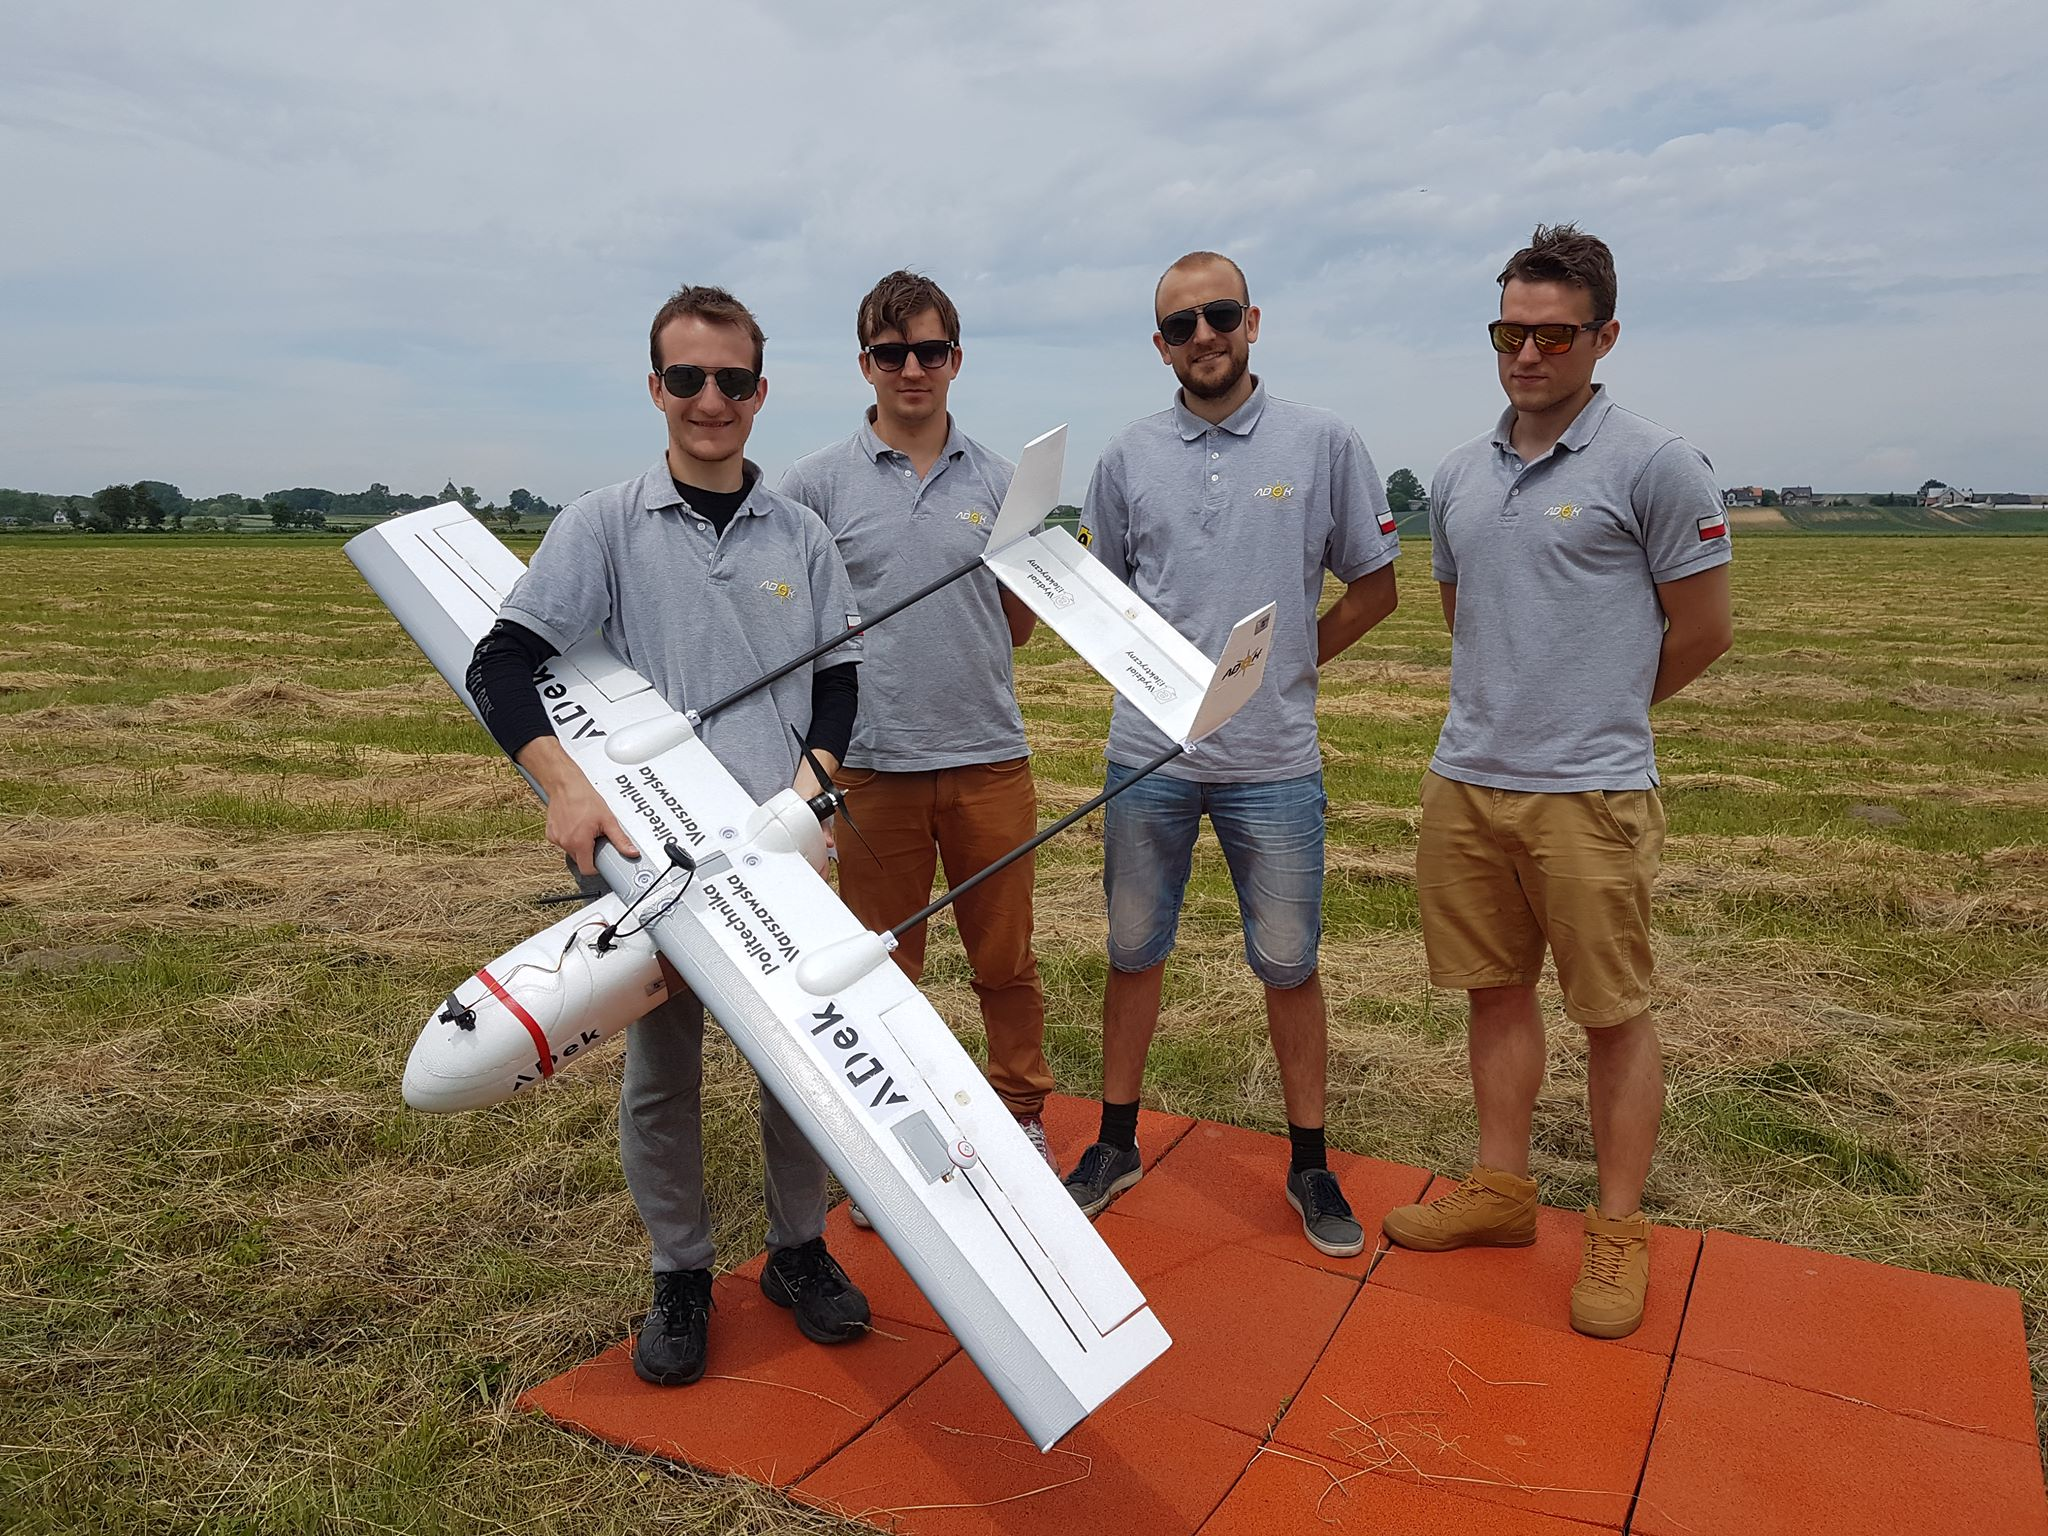
\includegraphics[width=15cm]{zalaczniki/obrazy/droniada.jpg}
    \caption{Nasz zespół na konkursie "Droniada".}
    \label{fig:triage}
\end{figure}

\subsection{Wprowadzenie do zagadnienia}
Projektowany system składał się z kliku części. Część pierwsza to poszkodowane w katastrofie osoby, którym ratownicy medyczni przypisują kolejne kolory przy pomocy beaconów, i tak kolor czerwony jest przyporządkowany do osób co do których wymagana jest natychmiastowa ewakuacja, kolorem żółtym oznaczone zostają osoby które wymagają pilnej ewakuacji (mniejszy priorytet), kolorem zielonym osoby które chodzą o własnych siłach, natomiast kolorem czarnym zgony, osoby których ciała zostaną usunięte dopiero po zakończeniu akcji ratowania życia. Jest to tzw. system znaczników Triage \cite{triage}.

\begin{figure}[!th]
    \centering
    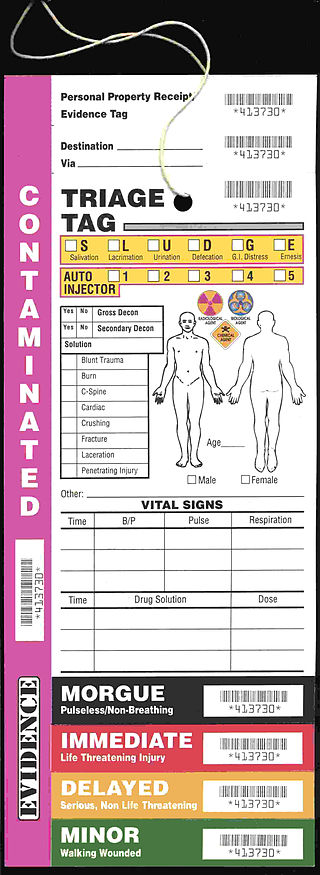
\includegraphics[width=5cm]{zalaczniki/obrazy/triage_tag.jpg}
    \caption{Typowy znacznik systemu Triage, używany w akcjach ratowniczych \cite{triage}.}
    \label{fig:triage}
\end{figure}

Kolejnym komponentem był statek powietrzny który miał za zadanie zbieranie, nadawanych dookólnie przez beacony, sygnałów i umiejscawianie ich na płaszczyźnie mapy. Taki statek musiał zostać wyposażony w odbiornik bluetooth w wersji conajmniej 4.0 i odpowiednie oprogramowanie.

Ostatnim elementem systemu był system naziemny (ang. \textit{Ground Station}). System ten zbierał zlokalizowane przez statek powietrzny sygnały i wyświetlał je na mapie, dodatkowo aproksymując pozycję realną beacona na mapie.

W kolejnych rozdziałach będę przybliżał powyższe komponenty systemu.

\section{Internet rzeczy}
\subsection{Koncepcja pomysłu internetu rzeczy}
Co to jest IoT, w jakim celu został stworzony, co nm daje.
\subsection{Sprzęt i BLE}
Z czego składa się IoT, jakich urządzeń używa, czym różni się bluetooth 4.0 od wcześniejszych wersji. Czym charakteryzują się kolejne wersji 4.1, 4.2, 4.3. Co to jest RSSI i jak je wykorzystać do określania pozycji, czy jest dokładne.
\subsection{Komponenty IoT wykorzystane w tworzonym systemie}
Beacony, gateway, urządzenia odbiorcze.

\section{Bezzałogowe statki powietrzne}
\subsection{Czym są UAV}
Bezzałogowy statek powietrzny, dron– statek powietrzny, który nie wymaga do lotu załogi obecnej na pokładzie oraz nie ma możliwości zabierania pasażerów, pilotowany zdalnie lub wykonujący lot autonomicznie...
\subsection{Rola UAV w projektowanym systemie}
Po co UAV, jak będziemy je wykorzystywać, czy nie lepiej skorzystać z czegoś innego.
\subsection{Autonomiczna misja}
Jak zaplanować, czy jest możliwa, jakie są obostrzenia, co mogę, a czego nie mogę zrobić w misji autonomicznej.
\subsection{Bezpieczeństwo stosowania UAV w misji ratunkowej}
Czy nie stanie się tak że trzeba będzie ratować ratownika, na co trzeba uważać, jak trzeba się oznaczyć, o czym należy pamiętać.

\section{Koncepcja techniczna systemu}
\subsection{Architektura tworzonego systemu}
Komponenty systemu, podział odpowiedzialności pomiędzy sprzęt i ludzi, protokoły pomiędzy urządzeniami, fale radiowe, zakłócenia...
\subsection{Schemat blokowy rozwiązania}
\subsection{Algorytm pracy}
Co po kolei się włącza, kto za co odpowiada i w którym momencie należy coś wyzwolić, pod jakimi warunkami, kto to ma zrobić.
\subsection{Podłączenie wielu statków w jeden system}
Czy jest możliwe, czy jest bezpieczne, jak nimi sterować, czy się wzajemnie nie zakłócają
\subsection{Sterowanie autonomiczne}
Jak to robić, jak unikać kolizji, jak plaować misje
\subsection{Bezpieczeństwo użytkowania}
O czym powienien pamiętać ratownik tak żeby sam nie potrzebował pomocy
\subsection{Aspekty mechaniczne systemu}

\section{Problemy i próba ich rozwiązania}
\subsection{Krótki czas lotu UAV}
\subsection{Zawodność linku telemetrycznego}
\subsection{Wrażliwość systemu na sytuacje wyjątkowe}
\subsection{Problemy sprzętowe}

\section{Testy systemu}
Loty autonomiczne, wyznaczanie charakterystyk siły sygnału bluetooth...

\section{Konkurs}
Jak nam poszło, jak dokładnie udało się określić pozycje, problemy podczas konkursu, wypadki, wyjątkowe sytuacje. Jak sprawdził się nasz osprzęt.

\section{Podsumowanie}
\subsection{Wnioski}
\subsection{Plany na przyszłość}

    \newpage
    %koniec treści głównej dokumentu

    %bibliografia
    \begin{thebibliography}{99}
 \bibitem{droniada}
 \emph{Parada Robotów Droniada 2017[online]}, dostęp w internecie w dniu 24 czerwca 2017:
 \url{http://www.5zywiolow.pl/droniada2017/}
 
 \bibitem{triage}
 \emph{Znacznik systemu Triage[online]}, dostęp w internecie w dniu 24 czerwca 2017:
 \url{https://en.wikipedia.org/wiki/Triage_tag}

 \bibitem{iot}
 \emph{Internet rzeczy[online]}, dostęp w internecie w dniu 24 czerwca 2017:
 \url{https://en.wikipedia.org/wiki/Internet_of_things}

\bibitem{ibeacon}
 \emph{Protokół iBeacon[online]}, dostęp w internecie w dniu 8 lipca 2017:
 \url{https://developer.apple.com/ibeacon/}

\bibitem{gateway}
 \emph{Gateway producji firmy kontakt.io[online]}, dostęp w internecie w dniu 8 lipca 2017:
 \url{https://store.kontakt.io/next-generation/33-gateway.html}

\bibitem{rtandroid}
 \emph{Strona domowa projektu RTAndroid[online]}, dostęp w internecie w dniu 8 lipca 2017:
 \url{https://rtandroid.embedded.rwth-aachen.de}

\end{thebibliography}
                       %polecenie programu WinEdt, włącza plik do drzewa 'projektu'
    \bibliographystyle{unsrtnat}                    %styl bibliografii: w kolejności cytowania, zrozumiały dla pakietu hyperref.sty
    \addcontentsline{toc}{section}{Literatura}      %musi być wyżej niż \bibliography{bibliografia}, żeby w~spisie treści był właściwy numer strony
    \bibliography{bibliografia}
    %koniec bibliografii


    %spis rysunków i~tablic
    %format spisu treści dotyczy tylko tych spisów, które są poniżej
    \hypersetup{linkcolor=black}
    \renewcommand{\cftparskip}{3pt}
    \clearpage
    \renewcommand{\cftloftitlefont}{\Large\bfseries\sffamily}
    \listoffigures
    \addcontentsline{toc}{section}{Spis rysunków}
    \renewcommand{\cftlottitlefont}{\Large\bfseries\sffamily}
    \listoftables
    \addcontentsline{toc}{section}{Spis tablic}
    \newpage
    %powrót do czerwonego koloru dla dalszych odnośników (spis literatury, przy włączonym pokazywaniu numerów stron, do których odnoszą się poszczególne pozycje)
    \hypersetup{linkcolor=red}

    %załączniki
    %\newpage
    %\appendix
    %\renewcommand{\appendixtocname}{Załączniki}
    %\renewcommand{\appendixpagename}{~\vspace{8cm} \begin{center}Załączniki\end{center}\newpage}
    %\thispagestyle{empty}
    %\addappheadtotoc
    %\appendixpage
    %\input{zalaczniki/tekstowe/schematSlave.tex}
\end{document}
